\section{Conclusie}
\label{sec:conclusie}

Na een evaluatie van de verschillende API architectuur vermeld in \autoref{sec:theoretisch kader}
en de eisen van het Robotica-project, is er tot de conclusie gekomen dat REST
de meest geschikte oplossing is.

De uiteindelijke UML diagram voor de API server is te zien in \autoref{fig:uml}.

\subsection{Overwegingen}
\label{ssec:overwegingen}
De belangrijkste punten die in overwegingen zijn genomen bij het kiezen van de
API architectuur waren:

\begin{enumerate}
    \item \textbf{Te ontwikkelen zonder libraries} --- Een van de vereisten van
     het project is dat de API server met zo min mogelijk libraries gemaakt moet
     worden.
    \item \textbf{Toegankelijkheid van de API} --- Het is essentieel dat de
     API eenvoudig te begrijpen en te gebruiken is. De API moest alle verzamelde
     data op een overzichtelijke manier kunnen presenteren.
    \item \textbf{Onderhoudbaarheid en Uitbreidbaarheid}: De API moet eenvoudig
    te onderhouden zijn, met een heldere en overzichtelijke structuur. Daarnaast
    moest de architectuur flexibel genoeg zijn om toekomstige uitbreidingen en
     aanpassingen te ondersteunen zonder dat de codebase herschreven moet worden.
\end{enumerate}

\subsection{Keuze voor REST}
Na het overwegen van de bovenstaande eisen en de doelen van het Robotica project,
is er uiteindelijk voor gekozen om REST te gebruiken door de volgende punten:

\begin{enumerate}
    \item \textbf{Eenvoudige implementatie} --- REST maakt gebruik van standaard
     HTTP/1.1-methoden, waardoor het gemakkelijk te implementeren is zonder de
     noodzaak van complexe frameworks of libraries. Hierdoor kan de API ontwikkeld
     worden met alleen een `TcpListener`.
    \item \textbf{Breed ondersteund en compatibel} --- Door zijn leeftijd
     ondersteund Vrijwel iedere webbrowser de infrastructuur waar REST op
     gebasseerd is, dit maakt het een ideale keuze voor toegankelijke
     webgebaseerde applicaties.
    \item \textbf{Flexibiliteit en uitbreidbaarheid} --- RESTful APIs kunnen
     eenvoudig worden uitgebreid met nieuwe functionaliteiten zonder bestaande
     endpoints te verstoren. Dit maakt het mogelijk om de API aan te passen aan
     eventuele nieuwe functies van het project.
\end{enumerate}

\subsection{Afweging tegen alternatieven}
\label{ssec:afweging tegen alternatieven}
Hoewel de alternatieve architecturen ook voordelen bieden over REST,
waren er enkele beperkingen die hen minder geschikt maakten voor dit project:

\begin{enumerate}
    \item \textbf{SOAP} --- Hoewel SOAP sterke beveiligingsfuncties biedt,
     werd het als te complex beschouwd voor de behoeften van dit project.
     De XML-gebaseerde berichten van SOAP introduceren heel wat overhead
     waardoor er meer ruimte voor fouten is.
    \item \textbf{GraphQL} --- Hoewel GraphQL veel flexibeler en efficiënter
     data kan opvragen dan REST, wordt er bij dit project geen gebruik gemaakt
     van grote set key-value paren, waardoor GraphQL overbodig is. Ook maakt de
     complexiteit het moeilijk om GraphQL te implementeren zonder bestaande
     library.
    \item \textbf{gRPC} --- gRPC biedt hoge prestaties en real-time communicatie,
     maar de complexiteit net zoals GraphQL en de beperkingen tot het gebruik
     van nieuwere browsers maakten het minder geschikt voor dit project.
\end{enumerate}

\subsection{UML model voor de API Server}
\label{ssec:uml model voor de api server}
\begin{figure}[H]
    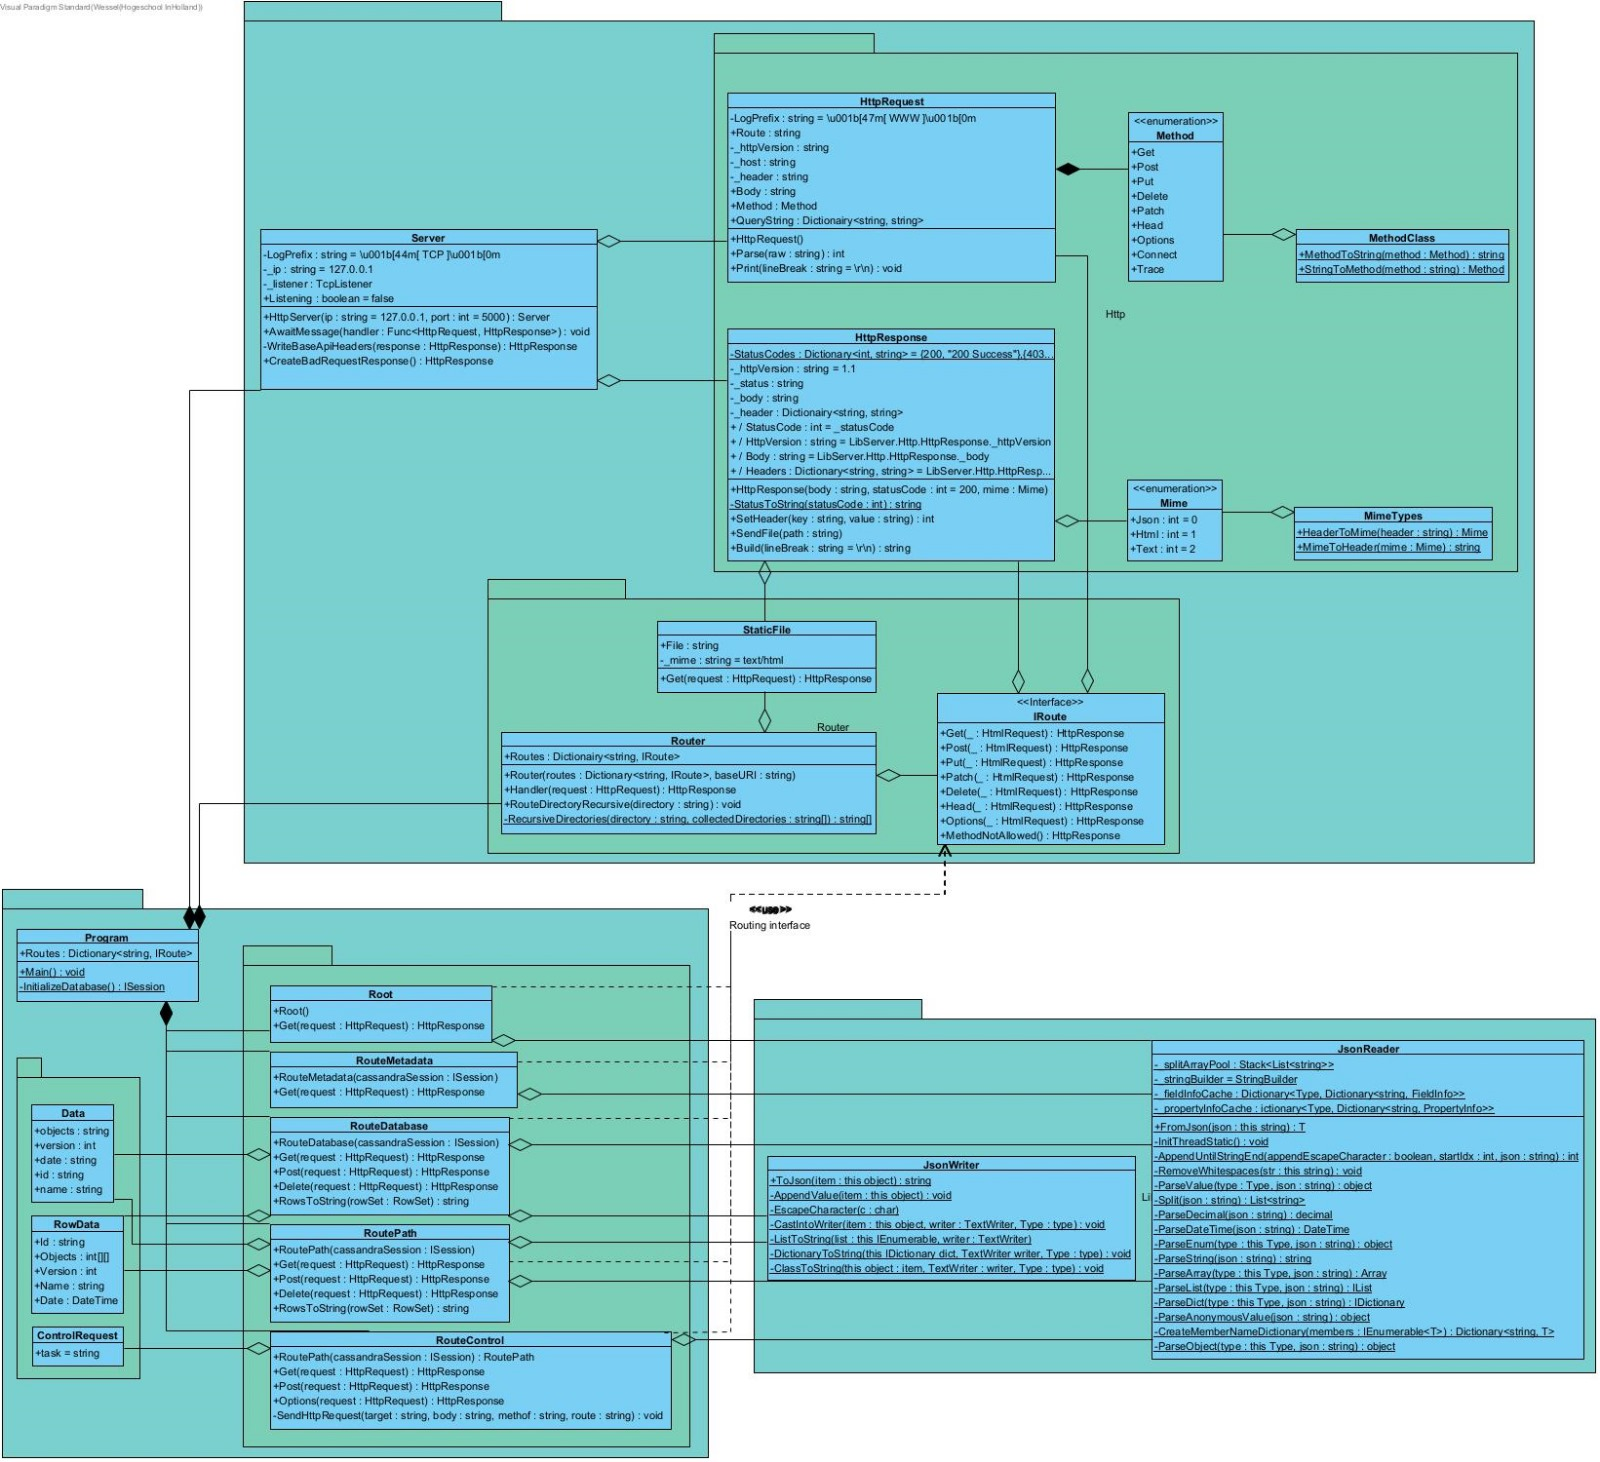
\includegraphics[width=0.5\textwidth]{uml.jpg}
    \caption{Resulterende UML voor de API server.}
    \label{fig:uml}
\end{figure}
